\documentclass{article}

\usepackage{times,fullpage,graphicx,amsmath, subfigure}
\usepackage[pdfborder={0 0 0}]{hyperref}

\title{Methpipe Manual}

\begin{document}
\maketitle
The Methpipe software package is a comprehensive tool chain for
analyzing whole genome bisulfite sequencing data (BS-Seq).  This
documentation will guide you step by step how to perform the
data analysis in a BS-Seq project with Methpipe. To facilitate
understanding of the work flow, we divide the analysis procedure into
four steps: (1) Pre-mapping processing includes assessing
read quality and  trimming adapters (if users use rmapbs for mapping, then 
trimming adapters as a separate step is not necessary); (2)
Mapping sequenced reads to a reference genome; (3)
Analyzing methylation level at a single site (CpG sites or
non-CpG cytosines). (4) Higher level analysis includes
identifying scores profiles (differential methylation or allelic methylation) 
and methylation characteristic regions (hypomethylated regions or 
differentially methylated regions). 

Next figure  shows detailed work flow of analysis with Methpipe.
Processes and corresponding tools are shown with rectangles: incoming and outgoing 
arrows represent the number of input and output files respectively.
Files with intermediate input or output data are shown as parallelograms
and files with the final results are shown as ovals.
The order of processes is important.
\begin{figure}[htbp]
  \centering
  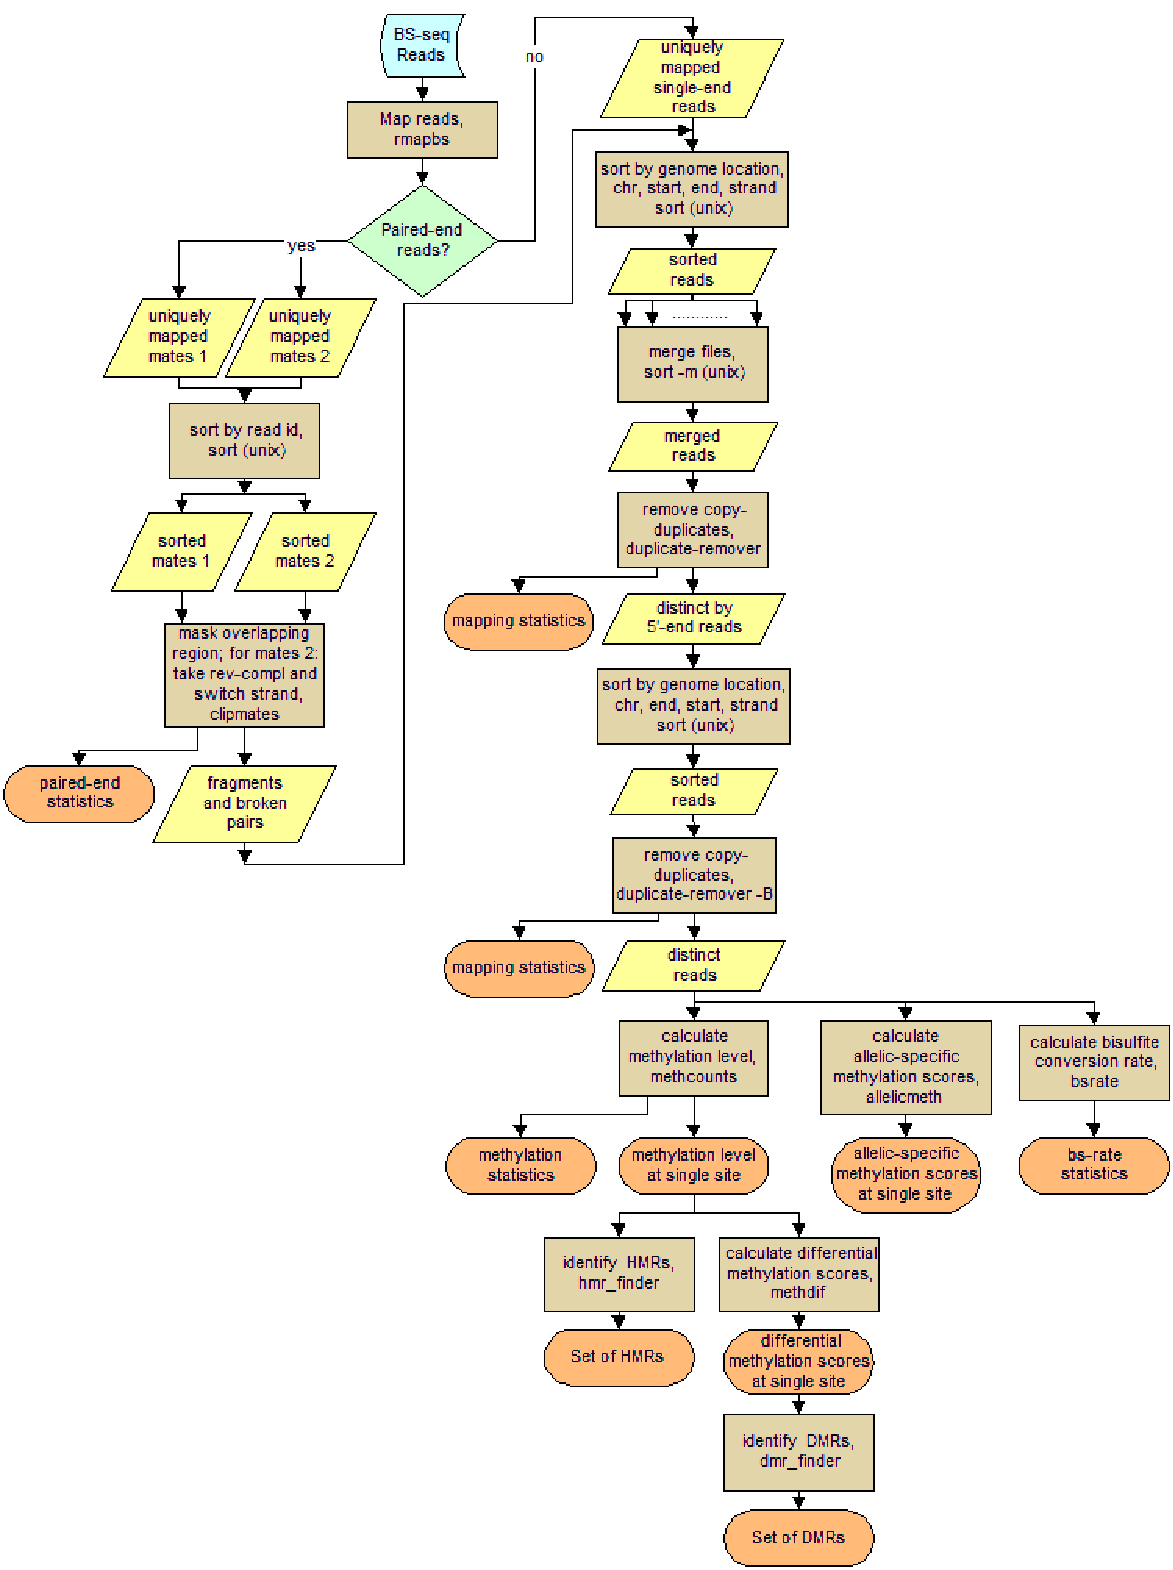
\includegraphics[width=6.3in]{figs/Methpipe_work_flow.pdf}
  \caption{Methpipe's Workflow}
  \label{fig:workflow}
\end{figure}
 
We will use provided test data as an example how to run our tools.
 Suppose that in
a project you would like to analyze methylomes of two
cell types, ESC and NHFF. There are paired-end sequenced reads for ESC
and single-end reads for NHFF: 
\begin{verbatim}
test_ESC_1.fastq, test_ESC_2.fastq, test_NHFF.fastq
\end{verbatim}
Two test references are in the directory \textit{test\_ref\_dir}.
We will discuss tools in the same order as they appear in Fig. \ref{fig:workflow}. For each
tool, we will describe what it does, the tool's options, and input/output formats.
Most of the tools use files in BED format and in Mapped Reads format, therefore we will provide these formats first, and 
later only refer to it by the name.


BED format:
\begin{itemize}
\item
reference name \textless string\textgreater
\item
start position within reference \textless integer\textgreater: starts with 0
\item
end position within reference \textless integer\textgreater: starts with 0
\item
name \textless string\textgreater : depends on the file (read ID, C-- content, HMR ID, DMR ID, etc.)
\item
score \textless float\textgreater : dependes on the file (number of mismatches, methylation level, score of HMR or DMR, etc.)
\item
strand \textless string\textgreater
\end{itemize}

Mapped Reads format:
\begin{itemize}
\item
reference name \textless string\textgreater
\item
start position within reference \textless integer\textgreater: starts with 0
\item
end position within reference \textless integer\textgreater: starts with 0
\item
name \textless string\textgreater : depends on the file (read ID, C-- content, HMR ID, DMR ID, etc.)
\item
score \textless float\textgreater : dependes on the file (number of mismatches, methylation level, score of HMR or DMR, etc.)
\item
strand \textless string\textgreater
\item
read \textless string\textgreater
\item
score \textless string\textgreater
\end{itemize}

\begin{flushleft}We will start with the tools for pre-mapping analysis (not shown in the workflow).
\end{flushleft}

\section{Pre-mapping processing}
\label{sec:premapping}
% \begin{description}
% \item[read-quality-prof.cpp]
% This program take a fastq file as input and output the base composition and 
% quality scores for each column
% \item[quality-prof.R]
% This R script define a function that takes the output of read-quality-prof.cpp as input 
% and draw the figure of base composition
% \item[trim-adapter.cpp] 
% This program expects a fastq file as input and trim the adapter sequence from the 3' end
% of reads if there is.
% \item[visireads.cpp]
% This program takes a fastq file as input and output a BED file displaying Cs in 
% the sequences
% \end{description}

Before mapping sequenced reads to a reference genome, we need to
pre-process the raw read sequences. In particular, we need to trim
adapter sequences retained in the 3' end of raw
reads. Further, we may be interested in examining the quality of reads
in our library and visualizing raw reads in UCSC Genome Browser. 

\subsection{Trim adapters}
\label{sec:trim-adapter}
As the length of sequenced reads
has been increasing all the time, it is possible there are adapter
sequences in the 3' end of some reads. These retained adapter
sequences affect the mappability of the reads. Even if the reads are
somehow mapped to the reference genome, the adapter sequences may
introduce bias to our estimate of methylation frequency. Therefore it
is necessary to trim these retained adapter sequences. 

The program \textbf{trim-adapter} is used to trim adapter sequences,
if any, from the 3' end of raw reads. Suppose the adapter sequence is
\textit{GATCGGAAGAGCGGTTCAGCAGGAATGCCGAGACCGATCTCGTATGCCG}, we mask
the adapter sequences from raw reads in the file
 \textit{test\_NHFF.fastq} with the
following command:
\begin{verbatim}
$ ./trim-adapter -o test_NHFF_adapter_masked.fastq   
-a GATCGGAAGAGCGGTTCAGCAGGAATGCCGAGACCGATCTCGTATGCCG test_NHFF.fastq  
\end{verbatim}

If you would like to know the effective read length distribution after trimming
adapter sequences and Ns from 3' end, you can add \textbf{-S} option
to specify the output file for the distribution of effective read lengths. For example,
\begin{verbatim}
./trim-adapter -a GATCGGAAGAGCGGTTCAGCAGGAATGCCGAGACCGATCTCGTATGCCG 
	       -S test_NHFF_read_length_distr.txt 
               -o test_NHFF_adapter_masked.fastq test_NHFF.fastq
\end{verbatim}
The file \textit{test\_NHFF\_read\_length\_distr.txt} contains distribution of effective reads
lengths after masking adapter sequences. Effective read length is the length of a read 
 without Ns at the end of the read.

While we provide this \textbf{trim-adapter} as a standalone program
for users who choose to map reads with another tool than rmapbs, its functionality is included
in the \textbf{rmapbs} tool.

OPTIONS:
\begin{itemize}
\item
\textbf{-a} \textless string\textgreater : adapter sequence
\item
\textbf{-o} \textless string\textgreater : output file (default: stdout) 
\item
\textbf{-S} \textless string\textgreater : output file with effective read length distribution
\item
\textbf{-N} : for counting effective read length (without this option effective length includes
the length of read without masked adapter sequence if any, and with this option it also includes
the length of read without Ns at the end of the read)
\end{itemize}

INPUT: reads in FASTQ format.

OUTPUT: reads in FASTQ format.

\subsection{Assessing read quality}
\label{sec:read-qual-assessm}
It is optional to assess read quality before mapping, however such
assessment may help us to spot potential problems during library
preparation and/or bisulfite sequencing. The program
\textbf{read-quality-prof} is used to generate an average summary of
base composition and quality scores from 5' to 3' along all
reads.  We run \textbf{read-quality-prof} as following 
\begin{verbatim}
$ ./read-quality-prof -o test_NHFF_qual.txt test_NHFF.fastq
\end{verbatim}

The output file \textit{test\_NHFF\_qual.txt} can be visualized with the R software.
Fig. \ref{fig:base-composition} shows the base composition profile in
the pair-end sequencing sample, where the left panel shows  T-rich
reads and the right panel A-rich reads. Note the small proportion of C
and G reflects the effect of bisulfite conversion.

\begin{figure}[htbp]
  \centering
\subfigure[T-rich reads]{
  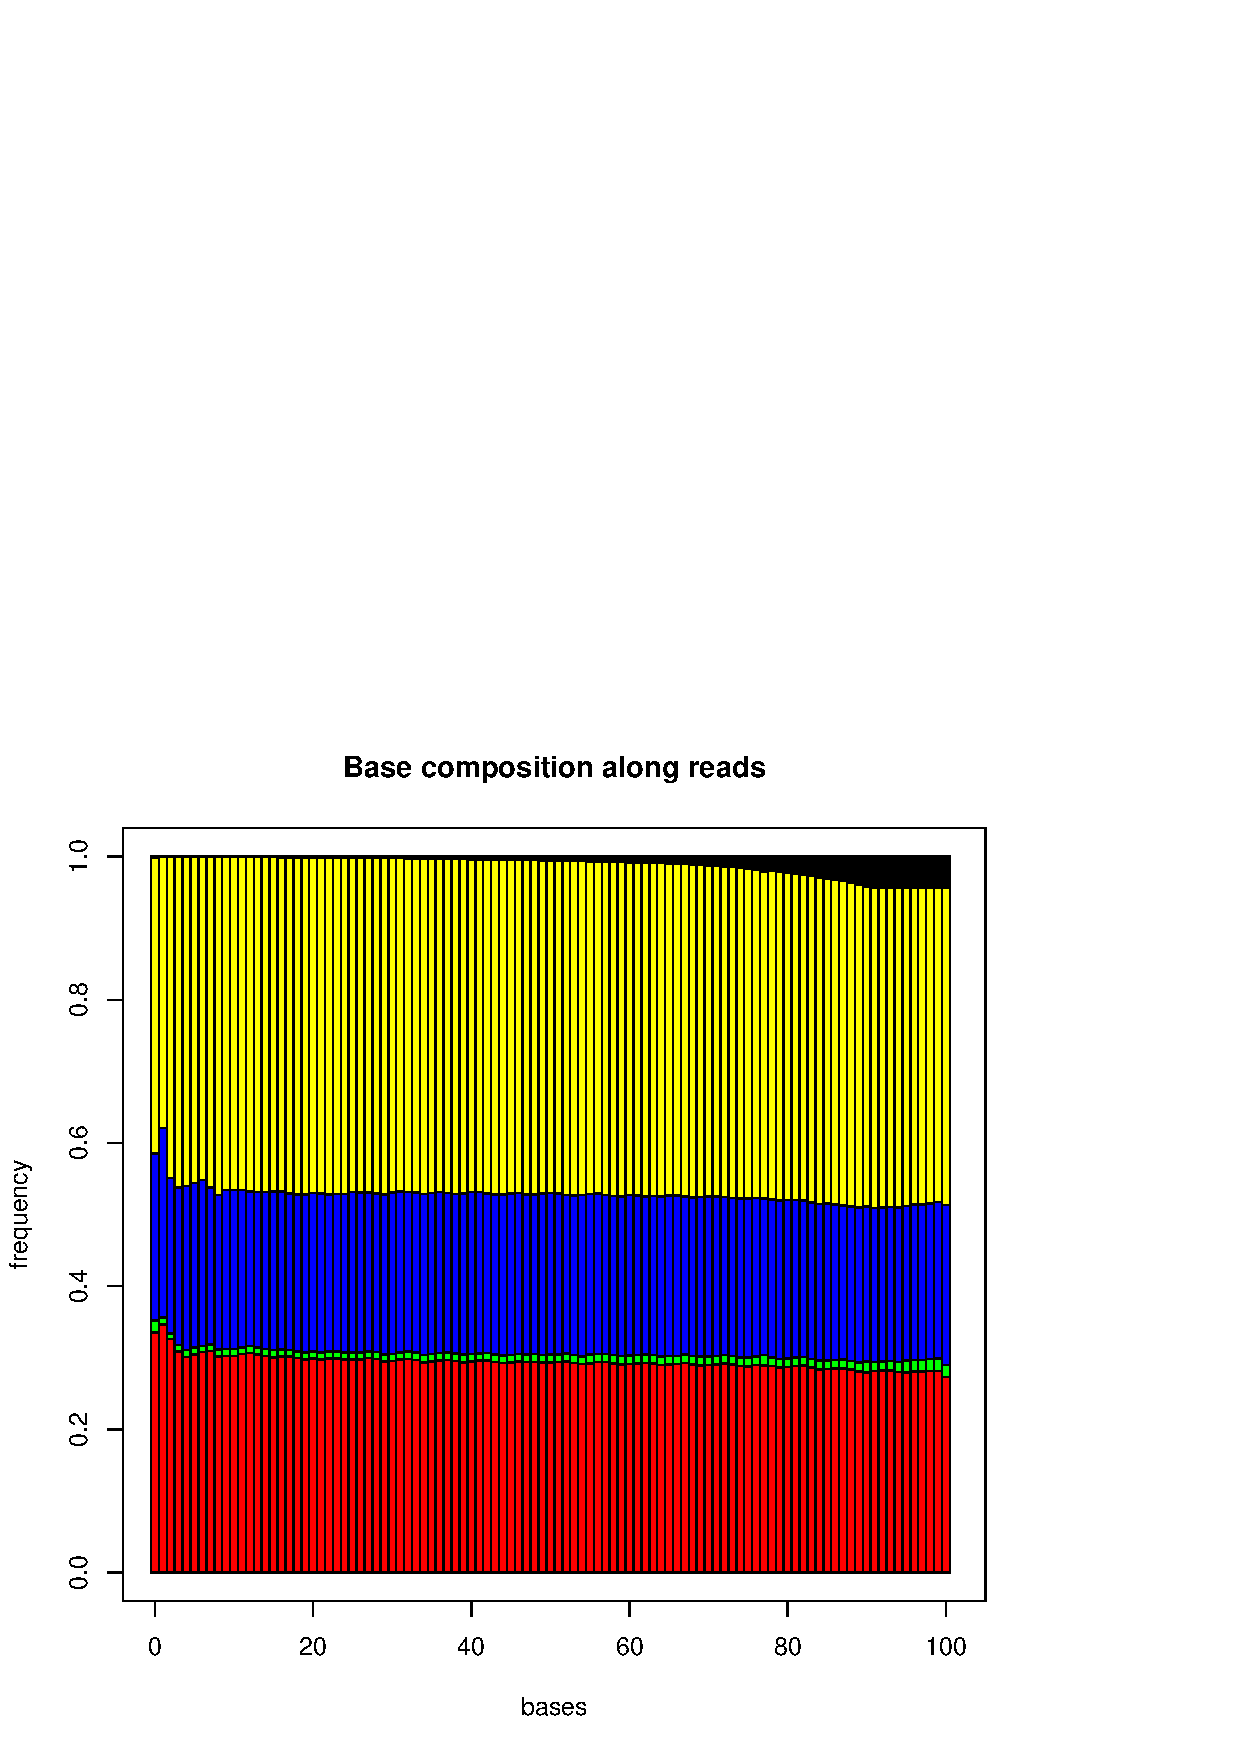
\includegraphics[width=2.8in]{figs/T-rich-base-composition.pdf}
}
\subfigure[A-rich reads]{
  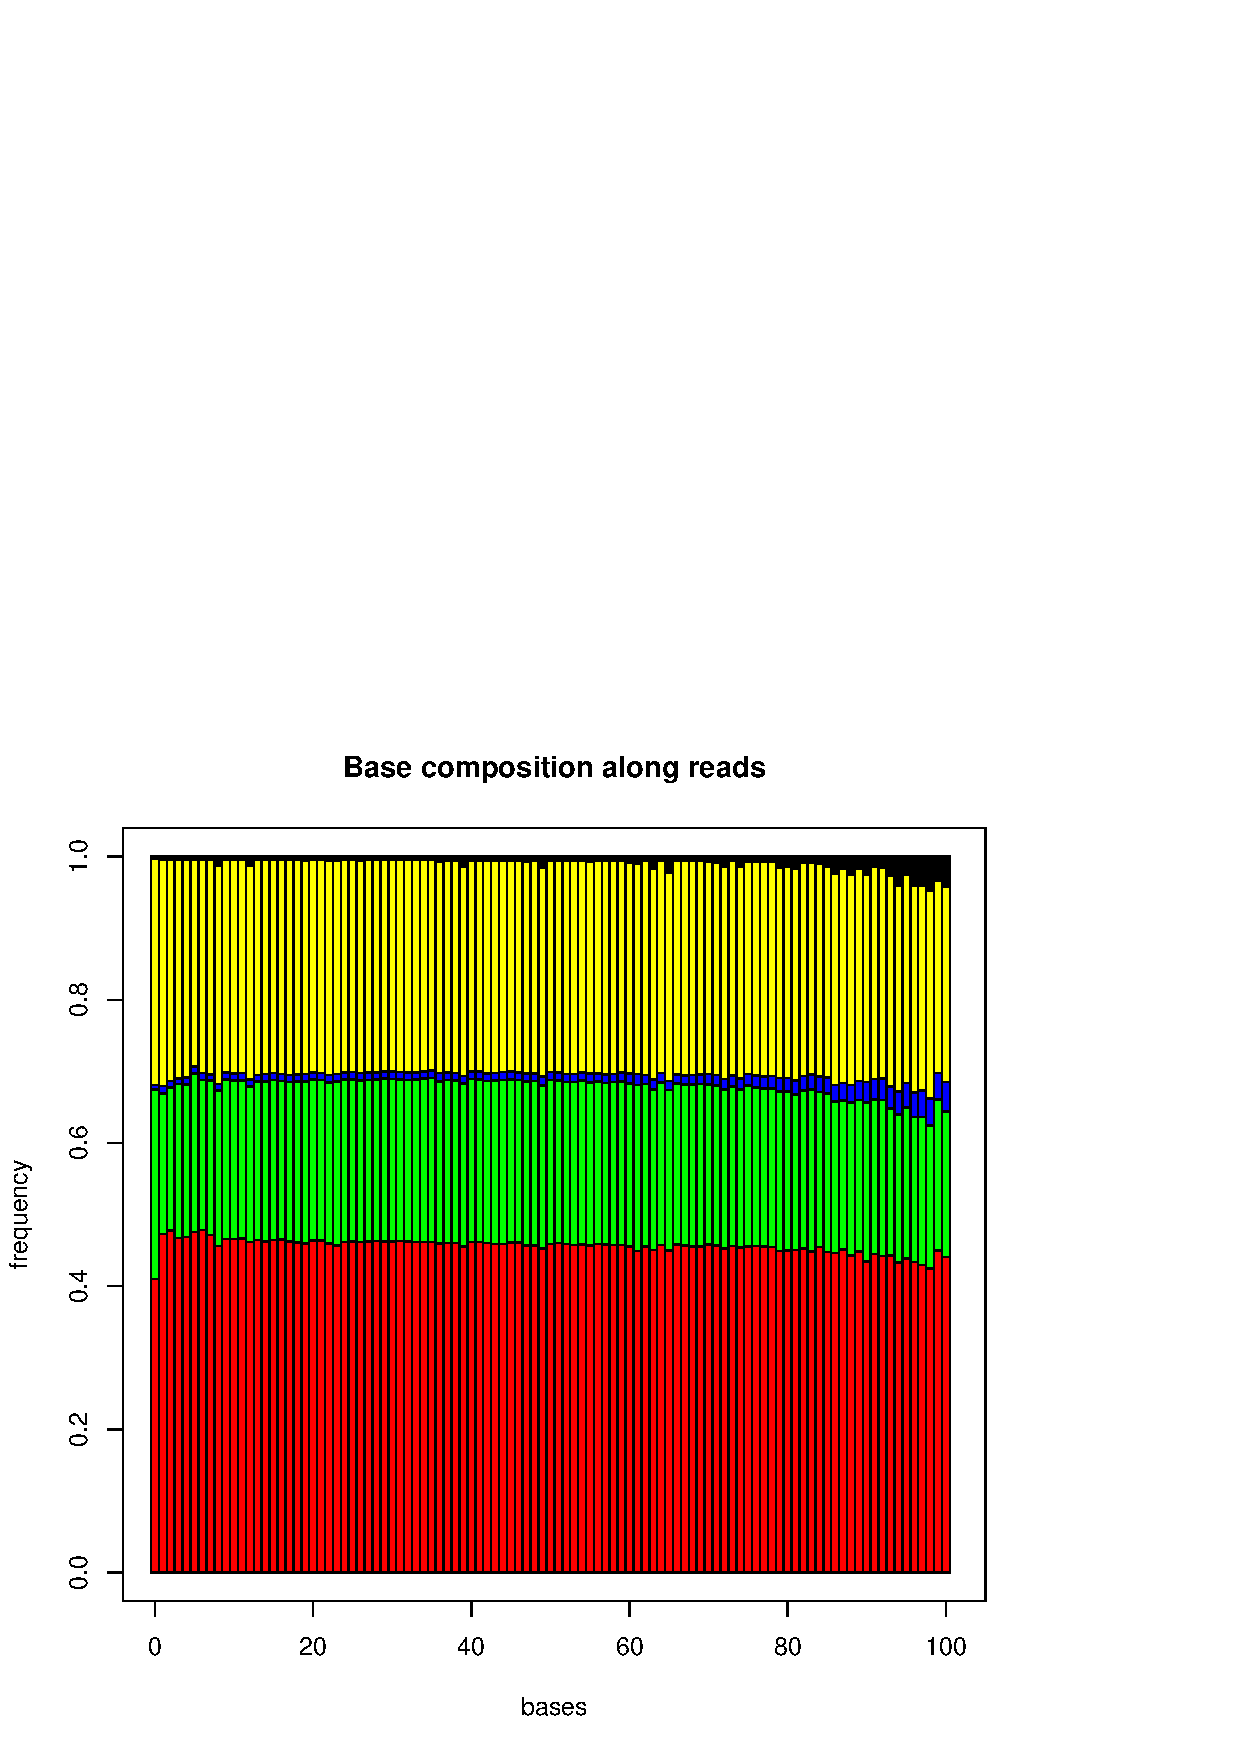
\includegraphics[width=2.8in]{figs/A-rich-base-composition.pdf}
}
  \caption{Base composition}
  \label{fig:base-composition}
\end{figure}

OPTIONS:
\begin{itemize}
\item
\textbf{-o} \textless string\textgreater : output file (default: stdout)
\end{itemize}

INPUT: reads in FASTQ format.

OUTPUT: self-explanatory column names are provided in the output file

\section{Mapping}
\label{sec:mapping}

% \begin{description}
% \item[rmapbs.cpp]
% This program takes fastq file as input and output mapped read file
% \end{description}

In the mapping step, you will map sequence reads to a reference
genome. During bisulfite treatment, unmethylated cytosines in the
original DNA sequences are converted to uracils, which are in turn
incorporated as thymines during PCR amplification. We call such strand
T-rich and its complementary strand A-rich (adenine-rich).  When
mapping T-rich reads to the reference genome, either a cytosine (C) or
a thymine (T) in reads is considered valid match to a cytosine in the
reference genome. But for A-rich reads, a adenine or a guanine is
consider valid match to a guanine in the reference genome.    

If using single-end sequencing, you will get T-rich reads only. If
using pair-end sequencing, you will get both T-rich reads and A-rich
reads (also referred to as $5^{\prime}$ end and $3^{\prime}$ mates respectively,
or as simply mates 1 and mates 2). 
Next we will learn how to map bisulfite treated reads with
\textbf{rmapbs} from either single-end sequencing or pair-end
sequencing. 

\subsection{Mapping single-end sequencing reads}
\label{sec:mapping-single-end}
Mapping read sequences to the reference genome is done by
\textbf{rmapbs}. To map paired-end reads, use \textbf{rmapbs} separately for 
$5^{\prime}$ end mates and for $3^{\prime}$ end mates. \textbf{IMPORTANT}:
use \textbf{-A} option when mapping mates 2. Failure to use option \textbf{-A}
with A-rich mates will result in mapping significantly less reads.

\begin{verbatim}
$ ./rmapbs -o test_ESC_1_mapped.mr -c test_ref_dir -m 3 -y test_ESC_1.fastq
$ ./rmapbs -o test_ESC_2_mapped.mr -c test_ref_dir -m 3 -y -A test_ESC_2.fastq
\end{verbatim}

\begin{flushleft} To map single end reads, run the command: \end{flushleft}
\begin{verbatim}
$ ./rmapbs -o test_NHFF_mapped.mr -c test_ref_dir -m 3 -y test_NHFF.fastq
\end{verbatim}

OPTIONS:
\begin{itemize}
\item
\textbf{-y} : allow N in read to match anything
\item
\textbf{-o} \textless string\textgreater : output file (default: stdout)
\item
\textbf{-c} \textless string\textgreater : FASTA file or directory containing files with chromosomes in 
	FASTA format (if option \textbf{-s} is not used, files with chromosomes must have
	\textbf{.fa} extension) 
\item
\textbf{-s} \textless string\textgreater : suffix of FASTA files (assumes -c indicates dir) 
\item
\textbf{-F} \textless string\textgreater : file listing names of chromosome files (absolute paths to
	chromosome files) 
\item
\textbf{-S} \textless integer\textgreater : number of seeds 
\item
\textbf{-h} \textless integer\textgreater : weight of hit 
\item
\textbf{-w} \textless integer\textgreater : width of the shortest reads in the input
\item
\textbf{-m} \textless integer\textgreater : maximum allowed mismatches 
\item
\textbf{-a} \textless string\textgreater : file to write names of ambiguously mapped reads 
\item
\textbf{-M} \textless integer\textgreater :  maximum allowed mappings for a read 
\item
\textbf{-W} : run in wildcard matching mode 
\item
\textbf{-P} \textless float\textgreater : wildcard cutoff probability 
\item
\textbf{-Q} : use quality scores (input must be FASTQ) 
\item
\textbf{-A} : map using A/G bisulfite wildcards (ALWAYS use with mates 2) 
\item
\textbf{-B} : allow CpG non-conversion to assist 
\item
\textbf{-f} : use faster seeds (sensitive to 2 mismatches) 
\item
\textbf{-C} \textless string\textgreater : clip the specified adaptor 
\item
\textbf{-v} : print more run info 
\item
\textbf{-G} : use original output format (BED)
\end{itemize}

INPUT: Reads are in FASTQ or FASTA format, and references are in FASTA format.

OUTPUT: Mapped Reads format.
 
\section{Post-mapping processing}
\label{sec:postmapping}

\subsection{Paired-end reads}
\label{sec:pairedend_reads}

Next we will discuss some necessary processing steps that are applied to
paired-end reads only.
As has been noted before, if using pair-end sequencing, you will get
both T-rich reads and A-rich reads. When estimating methylation
frequency of a cytosine residue, we count the number of cytosines,
which originate from methylated cytosines, and the number of thymines,
which originate from unmethylated cytosines, and then we use the ratio
$\frac{\#C}{\#C+\#T}$ as the estimate of methylation level of that
base. Since A-rich reads are complementary to the original DNA fragments, 
from which they were sequenced, A-rich reads reflect methylation status
of the cytosines on the strand, from which DNA fragments were originated.
To avoid a bias in calculating methylation level, A-rich reads need to be 
converted to T-rich reads
before we count Cs and Ts from these reads. 
Another bias in counting may arise from overlapping regions of two mates; to avoid
this we mask overlapping region in one mate with Ns preserving all valid information.
Conversion of A-rich reads to T-rich reads (taking reverse-complement of A-rich 
reads and switching the strand to which they mapped) and masking overlapping regions
is done by \textbf{clipmates}. This tool works on sorted by read id (read name) mapped
reads. 

To sort mapped paired-end reads by read id, use \textbf{sort (unix)}:
\begin{verbatim}
$ sort -k 4,4 test_ESC_1_mapped.mr > test_ESC_1_sortname.mr
$ sort -k 4,4 test_ESC_2_mapped.mr > test_ESC_2_sortname.mr
\end{verbatim}
\begin{flushleft}Then use \textbf{clipmates} that takes two input files: one
with T-rich mates and the other with A-rich mates.\end{flushleft}
\begin{verbatim}
$ ./clipmates -T test_ESC_1_sortname.mr -A test_ESC_2_sortname.mr
              -S test_ESC_clipmates_stat.txt -o test_ESC_clipmates.mr -L 500
\end{verbatim}
\begin{flushleft}This tool finds corresponding mates (whose names except for the last character
match), and if such mates exist and are mapped correctly (to the same chromosome, to
correct strands, with correct orientation) and within specified distance from each other
(option \textbf{-L}, maximum fragment size), then the mates are combined into 
a single fragment with Ns filled between the mates if there is a gap between them. If 
mates could not be matched, then each mate is present in the output. Thus, the output
file has Mapped Reads format and contains both entire DNA fragments or single mates.
Note that this tool takes reverse-complement and switches the strands for mates 2. \end{flushleft}

OPTIONS:
\begin{itemize}
\item
\textbf{-T} \textless string\textgreater : file with mates 1 (T-rich mates)
\item
\textbf{-A} \textless string\textgreater : file with mates 2 (A-rich mates)
\item
\textbf{-S} \textless string\textgreater : file with mapping statistics for paired-end reads
\item 
\textbf{-o} \textless string\textgreater : output file 
\item
\textbf{-L} \textless integer\textgreater : maximum length of DNA fragment (default: 1000)
\end{itemize}
 
INPUT: Two files with mates 1 and mates 2 in Mapped Reads format.

OUTPUT: Mapped Reads format with merged fragments and single mates. File with
paired-end mapping statistics has self-explanatory content.
 
\subsection{Paired-end and Single-end reads}
\label{sec:paired_single_reads}
During the post-mapping processign of mapped reads, we may need to
sort reads according to different criterions. This is done with the
\textbf{sort} utility provided in UNIX environment. 
Before calculating methylation level, users might consider removing
copy-duplicates, the reads that were mapped to the same genomic location and
 that most likely are by-product of PCR rather than representatives of 
two distinct DNA molecules. To remove copy-duplicates, users must aplly the following
steps: (1) sort reads by genomic location (chrom, start, end, strand), 
(2) merge files with reads that came from the same DNA library and the same PCR
and therefore likely to have shared copy-duplicates (3) run duplicate-remover 
that removes copy-duplicates mapped to the same start, (4)
sort reads by genomic location (chrom, end, start, strand), and (5)
run duplicate-remover with option \textbf{-B} that removes copy-duplicates
mapped to the same end positions. 

\begin{enumerate}
\item
Sort reads by genomic location: chrom, start, end, strand.
\begin{verbatim}
$ sort -k 1,1 -k 2,2g -k 3,3g -k 6,6 
       test_ESC_clipmates.mr > test_ESC_sorted_start.mr
$ sort -k 1,1 -k 2,2g -k 3,3g -k 6,6 
       test_NHFF_mapped.mr > test_NHFF_sorted_start.mr
\end{verbatim}
\item
Merge sorted files using \textbf{merge -m (unix)}. (We do not provide test data for this 
function)
\item
Run \textbf{duplicate-remover} to remove copy-duplicates sharing the same start position.
\begin{verbatim}
$ ./duplicate-remover -S test_ESC_duplremove_start_stat.txt
                      -o test_ESC_duplremove_start.mr  test_ESC_sorted_start.mr
\end{verbatim}
\item
Sort reads by genomic location: chrom, end, start, strand.
\begin{verbatim}
$ sort -k 1,1 -k 3,3g -k 2,2g -k 6,6 
       test_ESC_duplremove_start.mr > test_ESC_sorted_end.mr
$ sort -k 1,1 -k 3,3g -k 2,2g -k 6,6 
       test_NHFF_duplremove_start.mr > test_NHFF_sorted_end.mr
\end{verbatim}
\item
Run \textbf{duplicate-remover} to remove copy-duplicates sharing the same end position.
\begin{verbatim}
$ ./duplicate-remover -S test_ESC_duplremove_end_stat.txt
                       -o test_ESC_distinct.mr -B test_ESC_sorted_end.mr

$ ./duplicate-remover -S test_NHFF_duplremove_end_stat.txt
                       -o test_NHFF_distinct.mr -B test_NHFF_sorted_end.mr
\end{verbatim}
\end{enumerate}

The tool \textbf{duplicate-remover} collects reads and fragments mapped to the same
genomic location (start or end), and chooses a random one to be the representative of 
the original DNA fragment. If there are any fragments (both mates are mapped and matched, and 
merged into a fragment), then the representative is chosen from fragments. When considering
fragments mapped to the same genomic location, say fragments sharing same start, 
we treat fragments of different lengths as distinct DNA fragments. Below we provide options, 
and input/output format information for \textbf{duplicate-remover}.

OPTIONS:
\begin{itemize}
\item
\textbf{-o} \textless string\textgreater : output file
\item
\textbf{-S} \textless string\textgreater : file with mapping statistics
\item
\textbf{-B} : With paired-end reads duplicate-remover must be used twice. This option is used
	when we run duplicate-remover for the second time on reads sorted by chrom, end, start, strand.
	This option assumes this sorted order and removes copy-duplicates that share the same
	end position.
\end{itemize}

INPUT: A single file in Mapped Reads format.

OUTPUT: Output file is in Mapped Reads format and statistics file has self-explanatory output.

\section{Methylation level}
\label{sec:estim-methyl-freq}
% \begin{description}
% \item[methcount.cpp]
% This program reads mapped read file and output methylation frequency
% for each CpG site.
% \end{description}
The tool for calculating methylation level, \textbf{methcounts}, 
takes a single input file. Therefore, for a single methylome, users 
might need to merge multiple files from different libraries, and for this 
task please use \textbf{merge -m (unix)}.
In this section we will learn how to estimate the methylation
probability at a single cytosine loci. In mammals, DNA methylation
exists mostly at cytosines in the context of CpG dinucleotides. This
kind of methylation is symmetric because the cytosine on the
complementary strand, which is base-paired with the guanine, is also
methylated due to the interesting property of maintenance DNA
methyltransferases. In mammalian stem cells and in plant
cells, cytosines in sequence contexts other than CpG dinucleotides,
such as CHG or CHH (H denotes adenines, thymines or cytosines), may also be
methylated. This type of methylation is called asymmetric as the
cytosines on the complementary strand are unnecessarily
methylated. To calculate methylation level, use \textbf{methcounts}. 
This tool calculates methylation level for CpG sites by default; to calculate
methylation level for all cytosines, please use option \textbf{-N}.
\begin{verbatim}
$ ./methcounts -M 40 -c test_ref_dir 
               -o test_ESC_methcounts.bed test_ESC_distinct.mr
$ ./methcounts -N -M 40 -c test_ref_dir 
               -o test_NHFF_methcounts.bed test_NHFF_distinct.mr
\end{verbatim}

OPTIONS:
\begin{itemize}
\item
\textbf{-o} \textless string\textgreater : Output file (default: stdout) 
\item
\textbf{-c} \textless string\textgreater : FASTA file or directory containing chromosome(s) 
\item
\textbf{-s} \textless string\textgreater : suffix of FASTA files (assumes -c indicates dir) 
\item
\textbf{-N} : process non-CpG cytosines 
\item
\textbf{-B} \textless integer\textgreater : buffer size (in records, not bytes; default: 100000) 
\item
\textbf{-M} \textless integer or float\textgreater : max mismatches (can be fractional) 
\item
\textbf{-C} \textless float\textgreater : cutoff for high-quality bases (assumes fastq reads) 
\item
\textbf{-S} \textless string\textgreater : Output file with methylation statistics 
\item
\textbf{-v} : print more run info 
\end{itemize}

INPUT: A single file in Mapped Reads format.

OUTPUT: Output file is in BED format. File with statistics has self-explanatory content.
Field \textbf{name} has format \textbf{CpG:X}, where \textbf{CpG} is cytosine content and has 
three possible values, namely \textbf{CpG, CHH, CHG}, and \textbf{X} is the total number of 
Cs and Ts mapped to the site. Field \textbf{score} is methylation level.

\section{Estimating bisulfite conversion rate}
\label{sec:estim-busilf-conv}
By bisulfite sodiom treatment, unmethylated cytosines are converted to
uracils, which are later read out as thymines. However this conversion
may be incomplete due to various reasons, such as insufficient
concentration, insufficient time of treatment or sequencing
error. Therefore, bisulfite conversion rate, defined as ratio of
converted unmethylated cytosines to all unmethylated cytosines, is an
important parameter to assess the data quality of a BS-Seq
experiment. To stimate bisulfite conversion rate, we need first to
have some cytosines in the genome that are unmethylated. This includes
three scenarios: (i) non-CpG cytosines in most mammalian tissues, (ii)
spike-in Lamda genome and (iii) the chloroplast genome in plants. In
these three scenarios, unmethylated cytosines should all be converted
if the bisulfite treatment is perfect. Otherwise, some cytosines are
unchanged. Therefore we count the number of cytosines covering these
unmethylated cytosines and the number of thymines, the ratio of
thymines to cytosines and thymines combined is the estimator of the
bisulfite conversion rate.
To estimate bisulfite conversion rate in mammals (over non-CpG cytosines), run:
\begin{verbatim}
$ ./bsrate -c test_ref_dir -M 40 -o test_ESC_bsrate.txt test_ESC_distinct.mr
$ ./bsrate -c test_ref_dir -M 40 -o test_NHFF_bsrate.txt test_NHFF_distinct.mr
\end{verbatim}
\begin{flushleft}To estimate bisulfite conversion rate over all cytosines, use
option \textbf{-N}.\end{flushleft}

OPTIONS:
\begin{itemize}
\item
\textbf{-o} \textless string\textgreater : Output file with bs-rate statistics
\item
\textbf{-c} \textless string\textgreater : FASTA file or directory containing chromosome(s)
\item
\textbf{-s} \textless string\textgreater : suffix of FASTA files (assumes -c indicates dir) 
\item
\textbf{-N} : process all Cs
\item
\textbf{-B} \textless integer\textgreater : buffer size (in records; default: 100000)
\item
\textbf{-C} \textless integer\textgreater : cutoff for high-quality bases
\item
\textbf{-M} \textless integer\textgreater : max mismatches (can be fractional)
\item
\textbf{-v} : print more run info
\end{itemize}
 
INPUT: Mapped Reads format.

OUTPUT: Self-explanatory content.

\section{Higher level analysis}
\label{sec:high-level-analys}

\subsection{Allelic methylation scores}
\label{sec:allelic_scores}

We provide two tools to calculate methylation scores profiles. The tool \textbf{allelicmeth}
calculates allelic-specific methylation score for each CpG site. The higher score,
the more likely that the site has allelic-specific methylation. The allelic scores profile
can be visualized using a genome browser. Use the following command to generate 
allelic scores profile:
\begin{verbatim}
$ ./allelicmeth -M 40 -c test_ref_dir 
                -o test_ESC_allelicmeth.bed test_ESC_distinct.mr
$ ./allelicmeth -N -M 40 -c test_ref_dir 
                -o test_NHFF_allelicmeth.bed test_NHFF_distinct.mr
\end{verbatim}

OPTIONS:
\begin{itemize}
\item
\textbf{-o} \textless string\textgreater : Output file
\item
\textbf{-c} \textless string\textgreater : FASTA file or directory containing chromosome(s)
\item
\textbf{-s} \textless string\textgreater : suffix of FASTA files (assumes -c indicates dir)
\item
\textbf{-N} : process all Cs
\item
\textbf{-B} \textless integer\textgreater : buffer size (in records; default: 100000)
\item
\textbf{-C} \textless integer\textgreater : cutoff for high-quality bases
\item
\textbf{-M} \textless integer\textgreater : max mismatches (can be fractional)
\item
\textbf{-v} : print more run info
\end{itemize}

INPUT: Mapped Reads format.

OUTPUT FORMAT:
\begin{itemize}
\item
reference name \textless string\textgreater
\item
start position within reference \textless integer\textgreater: starts with 0
\item
end position within reference \textless integer\textgreater: starts with 0
\item
name \textless string\textgreater : in format \textbf{CpG:X}, where \textbf{X} is total number
of reads mapped to the site
\item
score \textless float\textgreater : allelic methylation score
\item
mm \textless integer\textgreater : total number of reads with methylation status of two consecutive CpGs methylated and methylated
\item
mu \textless integer\textgreater : total number of reads with methylation status of two consecutive CpGs methylated and unmethylated
\item
um \textless integer\textgreater : total number of reads with methylation status of two consecutive CpGs unmethylated and methylated
\item
uu \textless integer\textgreater : total number of reads with methylation status of two consecutive CpGs unmethylated and unmethylated
\end{itemize}

\subsection{Differential methylation scores}
\label{sec:methyldiff}

Our tool \textbf{methyldiff} generates differential methylation scores profile between
two methylomes. Given two methylomes (the result of \textbf{methcounts}), it calculates
the probability that a CpG is significantly less methylated in one methylome than in the other.
To generate differential methylation scores profile, run \textbf{methyldiff}:

\begin{verbatim}
$ ./methdiff -o test_NHFF_ESC_methdiff.bed 
             test_NHFF_methcounts.bed test_ESC_methcounts.bed
\end{verbatim}

OPTIONS:
\begin{itemize}
\item
\textbf{-o} \textless string\textgreater : Output file.
\item
\textbf{-p} \textless integer\textgreater : pseudocount for the contingency table
\item
\textbf{-v} : print more run info
\end{itemize}

INPUT: Two files in BED format, the results of \textbf{methcounts}.

OUTPUT: BED format file, with field \textbf{name} having format \textbf{CpG:X:Y}, 
where \textbf{X} is the total number of reads mapped to the site in one methylome, 
and \textbf{Y} is the total number of reads mapped to the site in the other methylome.
Field \textbf{score} contains differential methylation score.

\subsection{Hypomethylated regions, HMRs}
\label{sec:ident-hypo-methyl}

Hypomethylated regions, HMRs, are contiguous regions with very low methylation.
To identify HMRs, use the results of \textbf{methcounts} as input and run
\textbf{hmr\_finder}:
\begin{verbatim}
$ ./hmr_finder -i 20 -o test_ESC_HMR.bed test_ESC_methcounts.bed
$ ./hmr_finder -i 20 -o test_NHFF_HMR.bed test_NHFF_methcounts.bed
\end{verbatim}

OPTIONS:
\begin{itemize}
\item
\textbf{-o} \textless string\textgreater : Output file
\item
\textbf{-i} \textless integer\textgreater : maximum number of iterations 
\item
\textbf{-P} \textless string\textgreater : input file with parameters for HMM
\item
\textbf{-p} \textless string\textgreater : output file with parameters for HMM
\item
\textbf{-v} : print more run info 
\end{itemize}

INPUT: BED format file, results of \textbf{methcounts}.

OUTPUT: BED format file with HMRs.

\subsection{Differentially methylated regions, DMRs}
\label{sec:dmr}
Once differential methylation scores are calculated, the tool \textbf{dmr\_finder} can be
 used to identify differentially methylated regions, DMRs.
Option \textbf{-l} regulates the output: without this option, DMRs are calculated, in 
which methylation is less in one methylome, and with this option DMRs are calculated with methylation
less in the other methylome. Run \textbf{dmr\_finder} to identify DMRs.
\begin{verbatim}
$ ./dmr_finder -o test_NHFF_ESC_DMR.bed -d 500 -b 10 -C 10 -m 200 
               -c 0.7 test_NHFF_ESC_methdif.bed
\end{verbatim}

OPTIONS:
\begin{itemize}
\item
\textbf{-o} \textless string\textgreater : Output file
\item
\textbf{-b} \textless integer\textgreater : bandwidth in bases used for smoothing scores profile
\item
\textbf{-c} \textless float\textgreater : cutoff for peak confidence score
\item
\textbf{-C} \textless integer\textgreater : minimum number of CpGs per DMR
\item
\textbf{-m} \textless integer\textgreater : minimum size of DMR in bases
\item
\textbf{-l} : use lower cutoff (< 1 - cutoff)
\item
\textbf{-v} : print more run info
\end{itemize}

INPUT: BED format file, the result of \textbf{methdiff}.

OUTPUT: BED format file with DMRs.

\end{document}


